
Creating a library works similarly to creating an executable, although there are a few additional things to consider since library targets are usually used by other targets, either in the same project or by other projects. Since libraries usually have an internal part and a publicly visible API, we must take this into account when adding files to the project.

A simple project for a library will look like this:

\begin{lstlisting}[style=styleCMake]
cmake_minimum_required(VERSION 3.21)

project(
	ch3.hello_lib
	VERSION 1.0
	DESCRIPTION
	"A simple C++ project to demonstrate creating executables
	and libraries in CMake"
	LANGUAGES CXX)
	
add_library(hello)

target_sources(
	hello
	PRIVATE src/hello.cpp src/internal.cpp)
	
target_compile_features(hello PUBLIC cxx_std_17)

target_include_directories(
	hello
	PRIVATE src/hello
	PUBLIC include)
\end{lstlisting}

Again, the file starts with setting cmake\_minimum\_required and the project information, which should be familiar to you by now.

Next, the target for the library is created with add\_library – in this case, the type of the library is not determined. We could pass STATIC or SHARED instead to determine the linking type of the library explicitly. By omitting this, we allow any downstream consumers of the library to choose how to build and link it. Generally speaking, static libraries are the easiest to handle. More information about building shared libraries can be found in the Symbol visibility in shared libraries subsection. 

If the type of the library is omitted, the BUILD\_SHARED\_LIBS variable determines whether the libraries are built as shared or static libraries by default. This variable should not be set unconditionally in the CMake files of a project; it should always be passed by the user.

Next, the sources for the library are added with target\_sources. The first argument is the target name, followed by the sources separated by the PRIVATE, PUBLIC, or INTERFACE keyword. In practice, source files are almost always added with the PRIVATE specifier. The PRIVATE and PUBLIC keywords specify where the sources should be used for compiling. Specifying PRIVATE means that the sources will only be used in the target hello itself. If PUBLIC is used, then the sources will be added to hello and any target that links to hello. As we mentioned previously, this is not usually desired. The INTERFACE keyword would mean that the sources are not added to hello but should be added to anything that links against hello. Generally, anything that's specified as PRIVATE for a target can be seen as a build requirement. Finally, the include directories for the library are set using target\_include\_directories. All the files inside the folders specified by this command can be accessed using \#include <file.hpp> (with the angle brackets) instead of \#include "", although the version with the quotes may still work.

PRIVATE includes paths that will not be included in the target property; that is, INTERFACE\_INCLUDE\_DIRECTORIES. CMake will read this property when targets depend on the library to determine which of the include directories are visible to the dependee.

Since the C++ code of the library uses features that are tied to a modern version of C++ such as C++ 11/14/17/20 or C++ 23 (to be released soon), we must set the cxx\_std\_17 property. Since it is used to compile the library itself and to interface against the library, it is set to PUBLIC. Setting it to PUBLIC or INTERFACE is only necessary if the header files contain code that requires a certain standard. If only the internal code is dependent on a certain standard, setting it to PRIVATE is preferred. Generally, try to set the public C++ standard to the lowest that is working. It is also possible to only enable certain features of one of the modern C++ standards.

A full list of the available compile features can be found at \url{https://cmake.org/cmake/help/latest/prop_gbl/CMAKE\_CXX\_KNOWN\_FEATURES.html}.

\subsubsubsection{3.4.1\hspace{0.2cm}Naming libraries}

When you're creating libraries using add\_library(<name>), the name of the library must be globally unique inside the project as name collisions are errors. By default, the actual filename of the library is constructed according to the conventions on the platform, such as lib<name>.so on Linux and <name>.lib or <name>.dll on Windows. The name of the file can be changed from the default behavior by setting the OUTPUT\_NAME property of a target. This can be seen in the following example, where the name of the output file has been changed from ch3\_hello to hello:

\begin{lstlisting}[style=styleCMake]
add_library(ch3_hello)

set_target_properties(
	ch3_hello
	PROPERTIES OUTPUT_NAME hello
)
\end{lstlisting}

Avoid names for libraries with the prefix or postfix of lib as CMake may append or prepend the appropriate string to the filename, depending on the platform.

A frequently used naming convention for shared libraries is to add the version to the filename to specify the build version and API version. By specifying the VERSION and SOVERSION properties for a library target, CMake will create the necessary filenames and symlinks when building and installing the library:

\begin{lstlisting}[style=styleCMake]
set_target_properties(
	hello
	PROPERTIES VERSION ${PROJECT_VERSION} # Contains 1.2.3
	SOVERSION ${PROJECT_VERSION_MAJOR} # Contains only 1
)
\end{lstlisting}

On Linux, this example will result in a filename of libhello.so.1.0.0 with symlinks from libhello.so and libhello.so.1 pointing to the actual library file. The following screenshot shows the generated file and the symbolic links pointing to it:

\begin{center}
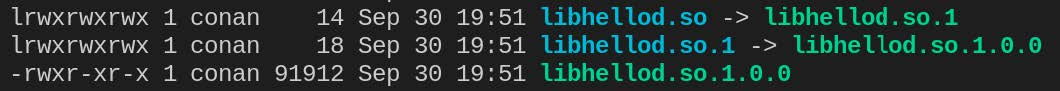
\includegraphics[width=1.\textwidth]{content/1/chapter3/images/1.jpg}\\
Figure 3.1 – The library file and the generated symlinks when building with the SOVERSION property
\end{center}

Another convention that's often seen in projects is adding a different postfix to the filename for the various build configurations. CMake handles this by setting the CMAKE\_<CONFIG>\_POSTFIX global variable to whatever the convention is or adding the <CONFIG>\_POSTFIX property to the targets. If this variable is set, the postfix will be automatically added to non-executable targets. As with most global variables, they should be passed to CMake over the command line or as a preset rather than hardcoded in the CMakeLists.txt file. 

The postfix for debug libraries can also be set explicitly to a single target, as shown in the following example:

\begin{lstlisting}[style=styleCMake]
set_target_properties(
hello
PROPERTIES DEBUG_POSTFIX d)
\end{lstlisting}

This will result in the library file and symlinks being named libhellod.so when you're building in the debug configuration. Since linking libraries is done over targets rather than filenames in CMake, picking the correct filename happens automatically, so we do not have to keep track manually. However, one thing to watch out for when linking shared libraries is symbol visibility. We'll look at this in the next section.

\subsubsubsection{3.4.2\hspace{0.2cm}Symbol visibility in shared libraries}

To link against shared libraries, the linker has to know which symbols can be used from outside the library. These symbols can be classes, functions, types, and more, and the process of making them visible is called exporting.

Compilers have different ways and default behavior when specifying symbol visibility, which makes specifying this in a platform-independent way a bit of a hassle. It starts with the default visibility of the compilers; gcc and clang assume that all the symbols are visible, while Visual Studio compilers, by default, hide all the symbols unless they're explicitly exported. By setting CMAKE\_WINDOWS\_EXPORT\_ALL\_SYMBOLS, the default behavior of MSVC can be changed, but this is a brute-force approach to the problem and can only be used if all the symbols of a library should be exported.

While setting all the symbols to publicly visible is an easy way to ensure that linking is easy, it has a few downsides:

\begin{itemize}
\item 
By exporting everything, there is no way of preventing the use of internal code by dependent targets.

\item 
Since every symbol can be used by external code, the linker cannot discard dead code, so the resulting libraries tend to be bloated. This is especially true if the library contains templates, which tend to blow up the number of symbols considerably.

\item 
Since every symbol is exported, the only clue about what should be considered hidden or internal has to come from the documentation.

\item 
Exposing the internal symbols of a library may expose things that should be kept hidden.

\hspace*{\fill} \\ %插入空行
\begin{tcolorbox}[colback=blue!5!white,colframe=blue!75!black,title=Setting All Symbols to Visible]
Be careful when you're setting all symbols to be visible in a shared library, especially when you're concerned about security issues or when the size of the binary is important.
\end{tcolorbox}
\end{itemize}

\hspace*{\fill} \\ %插入空行
\noindent
\textbf{Changing the default visibility}

To change the default visibility of the symbols, set the <LANG>\_VISIBILITY\_PRESET property to HIDDEN. This property can be set either globally or for a single library target. <LANG> is substituted for the language that the library is written in, such as CXX for C++ or C for C. If all the symbols are hidden symbols to be exported, they must be marked specially in the code. The most common way to do this is to specify a preprocessor definition that determines whether a symbol is visible or not:

\begin{lstlisting}[style=styleCXX]
class HELLO_EXPORT Hello {
	…
};
\end{lstlisting}

The HELLO\_EXPORT definition will contain information about whether the symbol will be exported when the library is compiled or whether it should be imported when you're linking against the library. GCC and Clang use the \_\_attribute\_\_(…) keyword to determine this behavior, while on Windows, \_declspec(…) is used. Writing header files that handle this in a cross-platform manner is not an easy task, especially if you also have to consider that libraries might be built as static and object libraries. Luckily, CMake provides the generate\_export\_header macro, which is imported by the GenerateExportHeader module, to make this easier.

In the following example, the symbols for the hello library are set to be hidden by default. Then, they are individually enabled again with the use of the generate\_export\_header macro, which is imported by the GenerateExportHeader module. Additionally, this example sets the VISIBILITY\_INLINES\_HIDDEN property to TRUE to further reduce the export symbol table by hiding inlined class member functions. Setting the visibility for inlines is not strictly necessary, but it's often done when the default visibility is set:

\begin{lstlisting}[style=styleCMake]
add_library(hello SHARED)
set_property(TARGET hello PROPERTY CXX_VISIBILITY_PRESET
	"hidden")
set_property(TARGET hello PROPERTY VISIBILITY_INLINES_HIDDEN
	TRUE)
include(GenerateExportHeader)
generate_export_header(hello EXPORT_FILE_NAME export/hello/
	export_hello.hpp)

target_include_directories(hello PUBLIC "${CMAKE_CURRENT_
	BINARY_DIR} /export")
\end{lstlisting}

The call to generate\_export\_header creates a file named export\_hello.hpp in the CMAKE\_CURRENT\_BINARY\_DIR/export/hello directory that can be included in the files of the library. It is good practice to put these generated files in a subfolder of the build directory so that only part of the directory is added to the include path. The include structure of the generated files should match the include structure of the rest of the library. So, if, in this example, all the public header files are included by calling \#include <hello/a\_public\_header.h>, the export header should also be placed in a folder called hello. The generated file also has to be added to the installation instructions, as explained in Chapter 4, Packaging, Deploying, and Installing a CMake Project. Additionally, to create the export file, the necessary compiler flags for exporting the symbols must be set to the target.

Since the generated header file must be included in the files that are declaring the classes, functions, and types to be exported, CMAKE\_CURRENT\_BINARY\_DIR/export/ is added to target\_include\_directories. Note that this has to be PUBLIC so that dependent libraries can find the file as well.

There are many more options regarding the generate\_export\_header macros, but what we have seen in this section covers the majority of use cases. Additional information about setting symbol visibility can be retrieved from the official CMake documentation at \url{https://cmake.org/cmake/help/latest/module/GenerateExportHeader.html}.

\subsubsubsection{3.4.3\hspace{0.2cm}Interface or header-only libraries}

Header-only libraries are a bit special as they are not compiled; instead, they export their headers so that they're directly included in other libraries. In most aspects, headeronly libraries work like normal libraries, but their header files are exposed using the INTERFACE keyword, rather than the PUBLIC keyword.

Since header-only libraries do not need to be compiled, they do not add sources to the targets. The following code creates a minimal header-only library:

\begin{lstlisting}[style=styleCMake]
project(
	ch3_hello_header_only
	VERSION 1.0
	DESCRIPTION "Chapter 3 header-only example"
	LANGUAGES CXX)

add_library(hello_header_only INTERFACE)
target_include_directories(hello_header_only INTERFACE
	include/)
target_compile_features( hello_header_only INTERFACE cxx_
	std_17)
\end{lstlisting}

It is also worth noting that before CMake version 3.19, the INTERFACE libraries could not have any target\_sources added. Now, header-only libraries can have no sources listed.

\hspace*{\fill} \\ %插入空行
\noindent
\textbf{Object libraries – for internal use only}

Sometimes, you may want to split off code so that parts of it can be reused without the need to create a full-blown library. A common practice is when you want to use some code in an executable and unit tests, without the need to recompile everything twice. For this, CMake provides object libraries, where the sources are compiled, but not archived or linked. An object library is created by calling add\_library(MyLibrary OBJECT).

Since CMake 3.12, these objects can be used like normal libraries by adding them to target\_link\_libraries functions. Before version 3.12, object libraries needed to be added with a generator expression; that is, \$<TARGET\_OBJECTS:MyLibrary>. This expands to a list of objects during build system generation. This can still be done, but it is no longer recommended as it quickly becomes unmaintainable, especially if there are multiple object libraries in a project.

\begin{tcolorbox}[colback=blue!5!white,colframe=blue!75!black,title=When to Use Object Libraries]
Object libraries help speed up building and modularizing code without making the modules public.
\end{tcolorbox}

With object libraries, all the different types of libraries are covered. Libraries on their own are fun to write and maintain, but unless they are integrated into a bigger project, they do not do anything. So, let's see how all the libraries we've defined so far can be used in an executable.








